\question (山东大学,05)下面程序段的时间复杂度为( ~) y=0;
while(n\textgreater{}=(y+1)*(y+1)) \{y++;\}
\par\fourch{}{}{\textcolor{red}{}}{}
\begin{solution}程序每次循环将y的值加1,然后比较n与y+1平方大小,所以总共要执行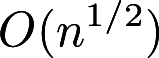
\includegraphics[width=0.57292in,height=0.20833in]{texmath/cb4bb05Cdpi7B3507DO28n5E7B12F27D29}次比较
\end{solution}
